\documentclass[twocolumn, 11pt]{article}
\usepackage{amsmath, amssymb, amsthm, bm, moresize}
\usepackage{euler}

\usepackage{graphicx, epsdice, xcolor, listings, float, wrapfig, caption}
\usepackage[top=1.2in, bottom=1.2in, left=0.6in, right=0.6in]{geometry}

\usepackage{etoolbox}
\patchcmd{\thebibliography}{\section*{\refname}}{}{}{}

\newcommand{\EE}{\mathbb{E}}
\newcommand{\PP}{\mathbb{P}}
\newcommand{\RR}{\mathbb{R}}
%
\newcommand{\Dd}{\mathcal{D}}
\newcommand{\Ee}{\mathcal{E}}
\newcommand{\Gg}{\mathcal{G}}
\newcommand{\Hh}{\mathcal{H}}
\newcommand{\Ii}{\mathcal{I}}
\newcommand{\Kk}{\mathcal{K}}
\newcommand{\Ll}{\mathcal{L}}
\newcommand{\Ss}{\mathcal{S}}
\newcommand{\Tt}{\mathcal{T}}
\newcommand{\Uu}{\mathcal{U}}
\newcommand{\Vv}{\mathcal{V}}
\newcommand{\Xx}{\mathcal{X}}
\newcommand{\Yy}{\mathcal{Y}}
%
\newcommand{\gG}{\frak{g}}
\newcommand{\oO}{\frak{o}}
\newcommand{\sS}{\frak{s}}


\newcommand{\Ein} {\text{trn}_{\Ss}} %{\Ee_{\text{in},\Uu}}
\newcommand{\Einb} {\text{trn}_{\check\Ss}} %{\Ee_{\text{in},\Uu}}
\newcommand{\Einc} {\text{trn}_{\Ss\sqcup \check\Ss}} %{\Ee_{\text{in},\Uu}}
\newcommand{\Egap}{\text{gap}_{\Ss}}
\newcommand{\Eout}{\text{tst}} %{\Ee_{\text{out}}}

\newtheorem*{qst}{Question}
\newtheorem*{thm}{Theorem}
\newtheorem*{lem}{Lemma}
\newtheorem*{clm}{Claim}
\theoremstyle{definition}
\newtheorem*{dfn}{Definition}

\definecolor{mblu}{rgb}{0.05, 0.40, 0.70}
\newcommand{\msec}[1]{\subsection*{\color{mblu}\textsf{#1}}}

\begin{document}

    \twocolumn[
        \begin{@twocolumnfalse}
            \begin{tabular}{p{0.06\linewidth}p{0.9\linewidth}}
                &
                \begin{flushleft}  \Huge \color{mblu} \bf\textsf{WHAT IS...}    \vspace{0.1cm}\\\hrule  \end{flushleft} \vspace{-1.0\baselineskip}
                \begin{flushright} \HUGE \color{mblu} \bf Stochastic Gradient Descent?   \end{flushright} \vspace{-1.0\baselineskip}
                \begin{flushright} \Large             \it Samuel C.\ Tenka      \end{flushright}
            \end{tabular}
        \end{@twocolumnfalse}
    ]

    \msec{Optimization}
    \msec{The Metric's Role}
        Representer Theorem
    \msec{}
    \msec{}

    \msec{References}
        We thank \textsc{Sho Yaida} for teaching us that physics is everywhere.

        \hrulefill
        \vspace{0.4cm}
            \begin{wrapfigure}{r}{3.3cm}
                \vspace{-0.4cm}
                    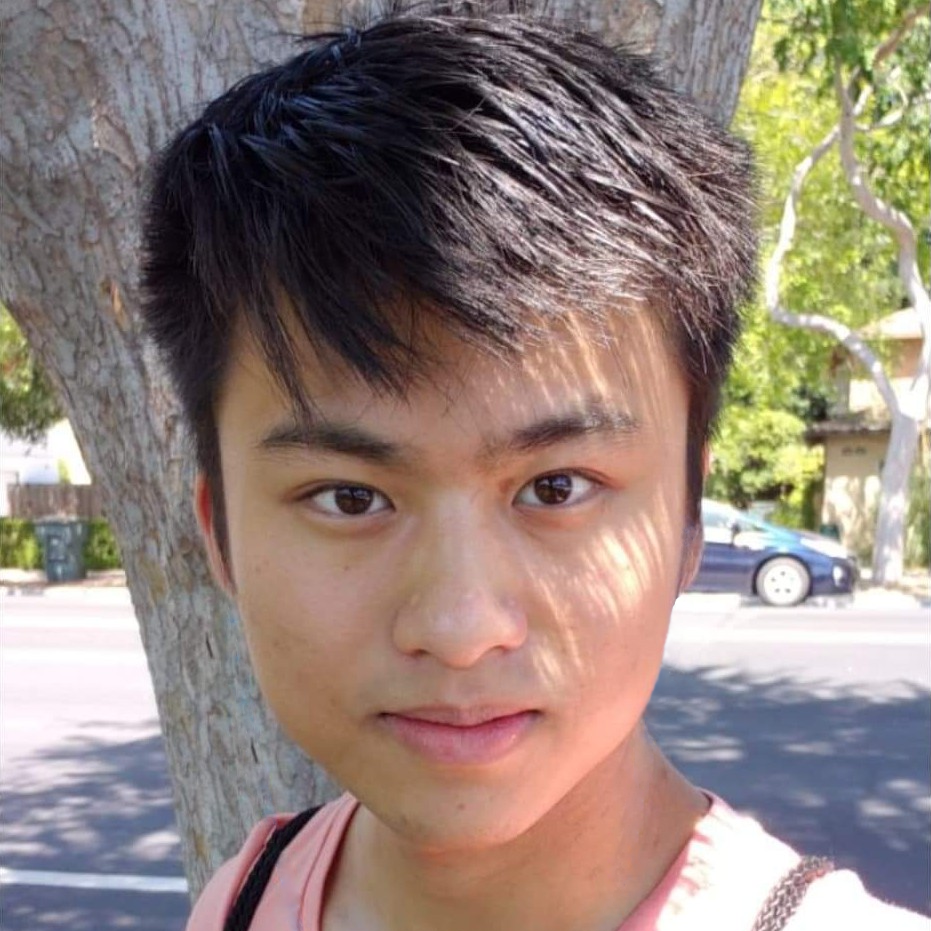
\includegraphics[height=3.3cm]{sam}
                \caption*{The author, courtesy of Karl Winsor}
            \end{wrapfigure}
            When not thinking about machines that learn, Sam can often be found
            pretending to be a cow.  Sam enjoys memory over experience, pet
            snails over pet spinach, left adjoints over right adjoints, and
            analogies over lists.


\end{document}


